\documentclass{beamer}
\usetheme{metropolis}

\setbeamercolor{background canvas}{bg=white}

\usepackage[spanish]{babel}
\usepackage[utf8]{inputenc} % Codificación UTF-8
\usepackage{lmodern} % Fuente moderna para LaTeX

\title{Multi-modal recommender system for\\content streaming platforms}
\subtitle{Trabajo Final del Máster en Ciencia de Datos\\
Universitat Oberta de Catalunya}
\date{\today}
\author{José María Tagarro Martí}
\institute{Area: Data science in complex systems, sustainability and ecology\\Tutor: Francesc Julbe López\\Profesora: Susana Acedo Nadal}

\begin{document}

% Portada
\maketitle

% Índice
\begin{frame}{Índice}
    \tableofcontents
\end{frame}

% Introduction
\section{Introducción}
\begin{frame}{Contexto y motivación}
    \textbf{¿Por qué los sistemas de recomendación son esenciales para una plataforma de \textit{streaming}?}
    \begin{itemize}
        \item Buscar contenidos en una TV con un catálogo de miles de títulos es frustrante.
        \item Problemas clave:
            \begin{itemize}
                \item Escalabilidad para miles de títulos y millones de usuarios.
                \item \textit{Cold start}: dificultad para recomendar a nuevos usuarios o elementos.
                \item \textit{Long tail}: subrepresentación de contenido menos popular.
            \end{itemize}
    \end{itemize}
\end{frame}

% Problem Description
\section{Descripción del problema}
\begin{frame}{Problema de la larga cola}
    \begin{figure}
        \centering
        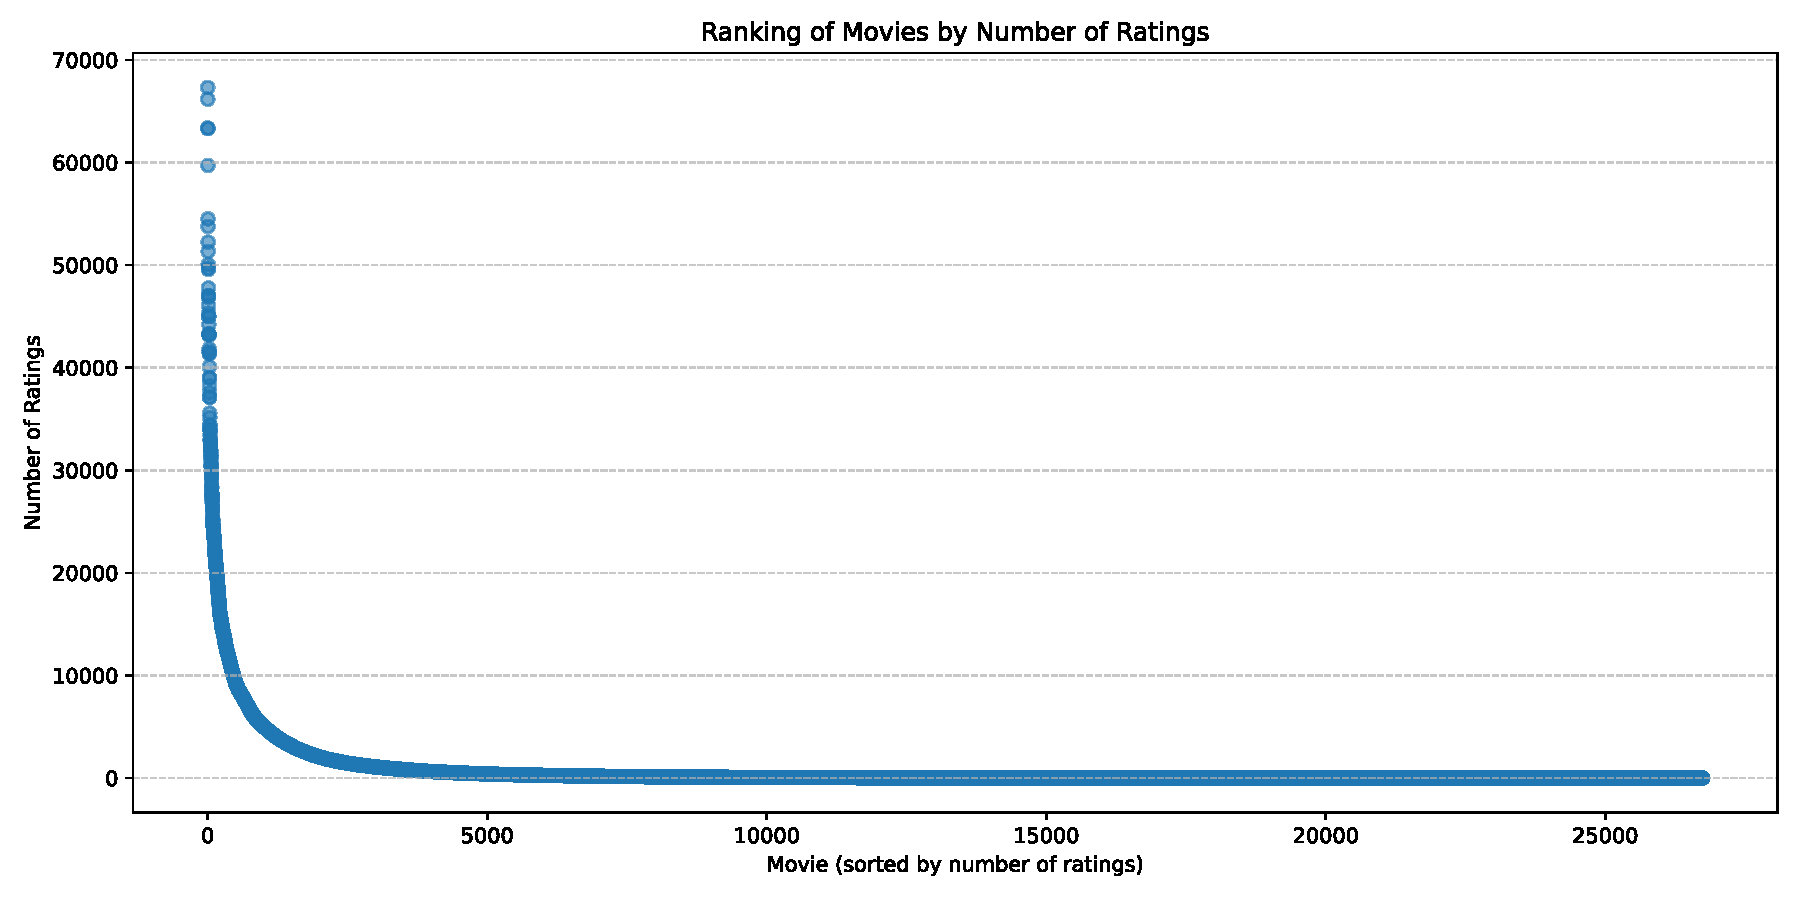
\includegraphics[width=\textwidth]{images/ranking_of_movies_by_ratings.pdf}
    \end{figure}
\end{frame}

% Goals and Contributions
\section{Objetivos y contribuciones}
\begin{frame}{Objetivos y contribuciones}
    \textbf{Objetivo principal:} Implementar un sistema de recomendación multimodal. \\
    \vspace{0.5cm}
    \textbf{Contribuciones clave:}
    \begin{itemize}
        \item Primera aplicación de DMRL en plataformas de streaming.
        \item Creación de un dataset extendido basado en MovieLens-20M con subtítulos y pósters.
        \item Exploración del impacto de las nuevas modalidades en los problemas de \textit{cold start} y \textit{long tail}.
    \end{itemize}
\end{frame}

% Dataset Description
\section{Descripción del dataset}
\begin{frame}{Proceso de integración del dataset}
    \begin{figure}
        \centering
        \usetikzlibrary{positioning, arrows.meta, shadows}
        \begin{tikzpicture}[
            scale=0.5, transform shape,
            node distance=0.75cm and 1cm,
            process/.style={rectangle, fill=white, drop shadow, draw, minimum width=3cm, align=center, minimum height=1.5cm},
            dataset/.style={rectangle, fill=white,  drop shadow, draw, minimum width=3cm, align=center, minimum height=1.5cm},
            output/.style={rectangle, fill=white,  drop shadow, draw, minimum width=3cm, align=center, minimum height=8.25cm},
            arrow/.style={-{Stealth}}
        ]
        
        % Datasets
        \node[dataset] (movielens) {MovieLens};
        \node[dataset, below=of movielens] (posterlens) {PosterLens};
        \node[dataset, below=of posterlens] (sublens) {SubLens};
        \node[dataset, below=of sublens] (tmdb) {TMDB};
        
        % Processes for MovieLens
        \node[process, right=of movielens] (ml_id_matching) {Match\\IDs};
        
        % Processes for PosterLens
        \node[process, right=of posterlens] (pl_id_matching) {Match\\IDs};
        \node[process, right=of pl_id_matching] (pl_resizing) {Resize\\Images};
        \node[process, right=of pl_resizing] (pl_feature_extraction) {Extract\\Features};
        
        % Processes for SubLens
        \node[process, right=of sublens] (sl_id_matching) {Match\\IDs};
        \node[process, right=of sl_id_matching] (sl_transform) {Plaintext};
        \node[process, right=of sl_transform] (sl_numpy) {NumPy Array};
        
        % Processes for TMDB Metadata
        \node[process, right=of tmdb] (tmdb_id_matching) {Match\\IDs};

        % Integrated node
        \node[output, right=10cm of tmdb_id_matching, yshift=3.5cm] (ml_output) {MovieLens\\Composite\\Multi-modal\\Dataset};
        
        % Arrows for MovieLens
        \draw[arrow] (movielens) -- (ml_id_matching);
        \draw[arrow] (ml_id_matching) -- (ml_id_matching-|ml_output.west);
        
        % Arrows for PosterLens
        \draw[arrow] (posterlens) -- (pl_id_matching);
        \draw[arrow] (pl_id_matching) -- (pl_resizing);
        \draw[arrow] (pl_resizing) -- (pl_feature_extraction);
        \draw[arrow] (pl_feature_extraction) -- (pl_feature_extraction-|ml_output.west);
        
        % Arrows for SubLens
        \draw[arrow] (sublens) -- (sl_id_matching);
        \draw[arrow] (sl_id_matching) -- (sl_transform);
        \draw[arrow] (sl_transform) -- (sl_numpy);
        \draw[arrow] (sl_numpy) -- (sl_numpy-|ml_output.west);
        
        % Arrows for TMDB Metadata
        \draw[arrow] (tmdb) -- (tmdb_id_matching);
        \draw[arrow] (tmdb_id_matching) -- (tmdb_id_matching-|ml_output.west);
        
        \end{tikzpicture}
    \end{figure}
\end{frame}

% Model Description
\section{Descripción del modelo}
\begin{frame}{¿Qué es \textit{disentangled representation learning}?}
    \begin{figure}
        \centering
        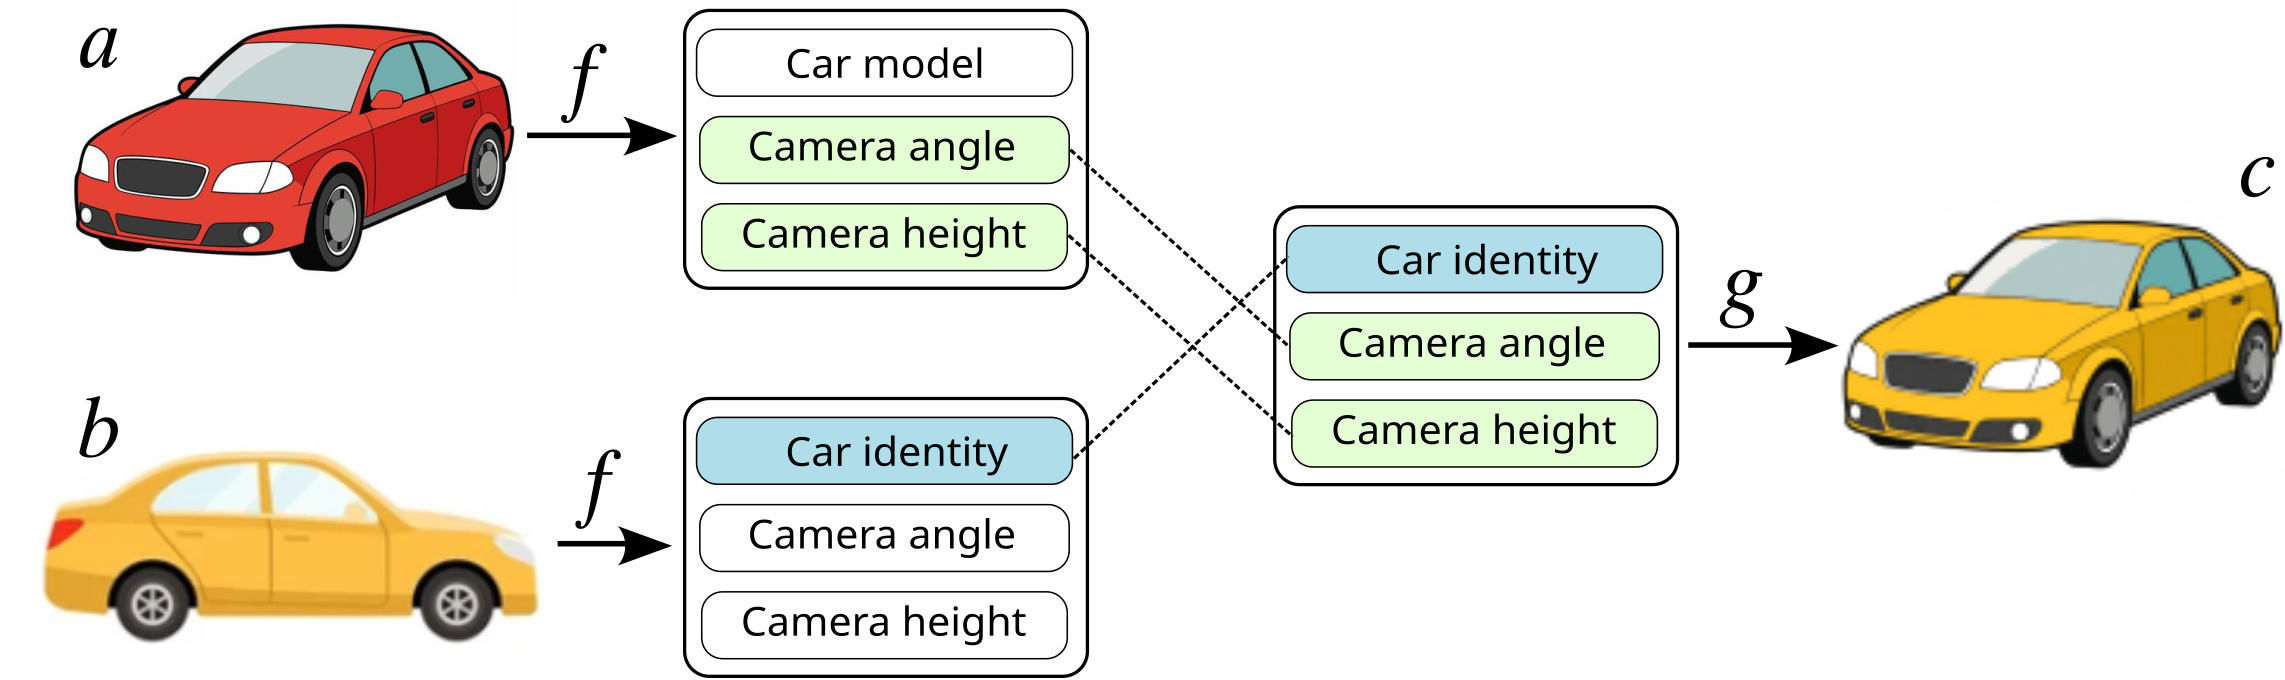
\includegraphics[width=0.9\textwidth]{images/disentangled-representation-learning.png}
    \end{figure}
\end{frame}

\begin{frame}{Arquitectura de DMRL}
    \begin{figure}
        \centering
        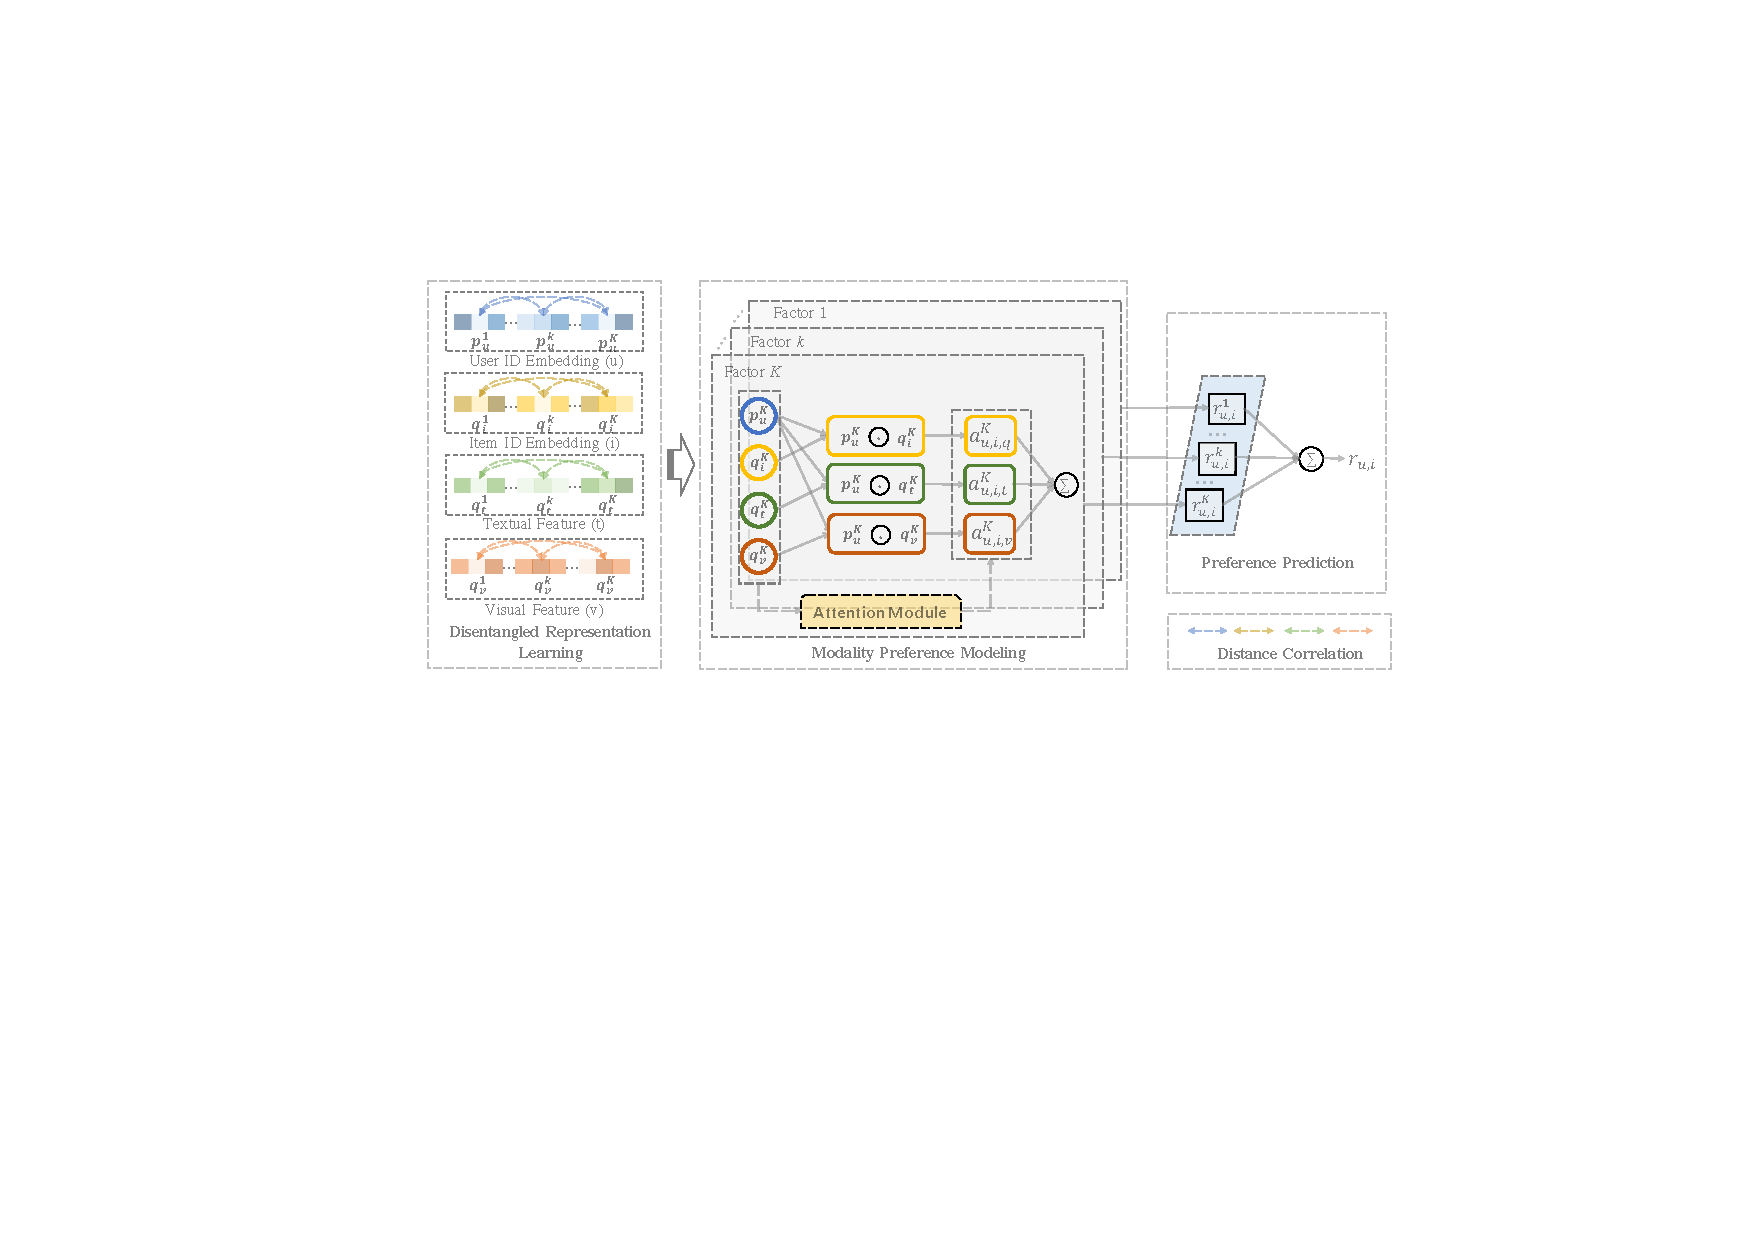
\includegraphics[width=0.9\textwidth]{images/dmrl_arch.pdf}
    \end{figure}
\end{frame}

% Experimental Results
\section{Resultados experimentales}
\begin{frame}{Comparación de NDCG y Recall}
    \begin{figure}
        \centering
        \begin{minipage}{0.48\textwidth}
            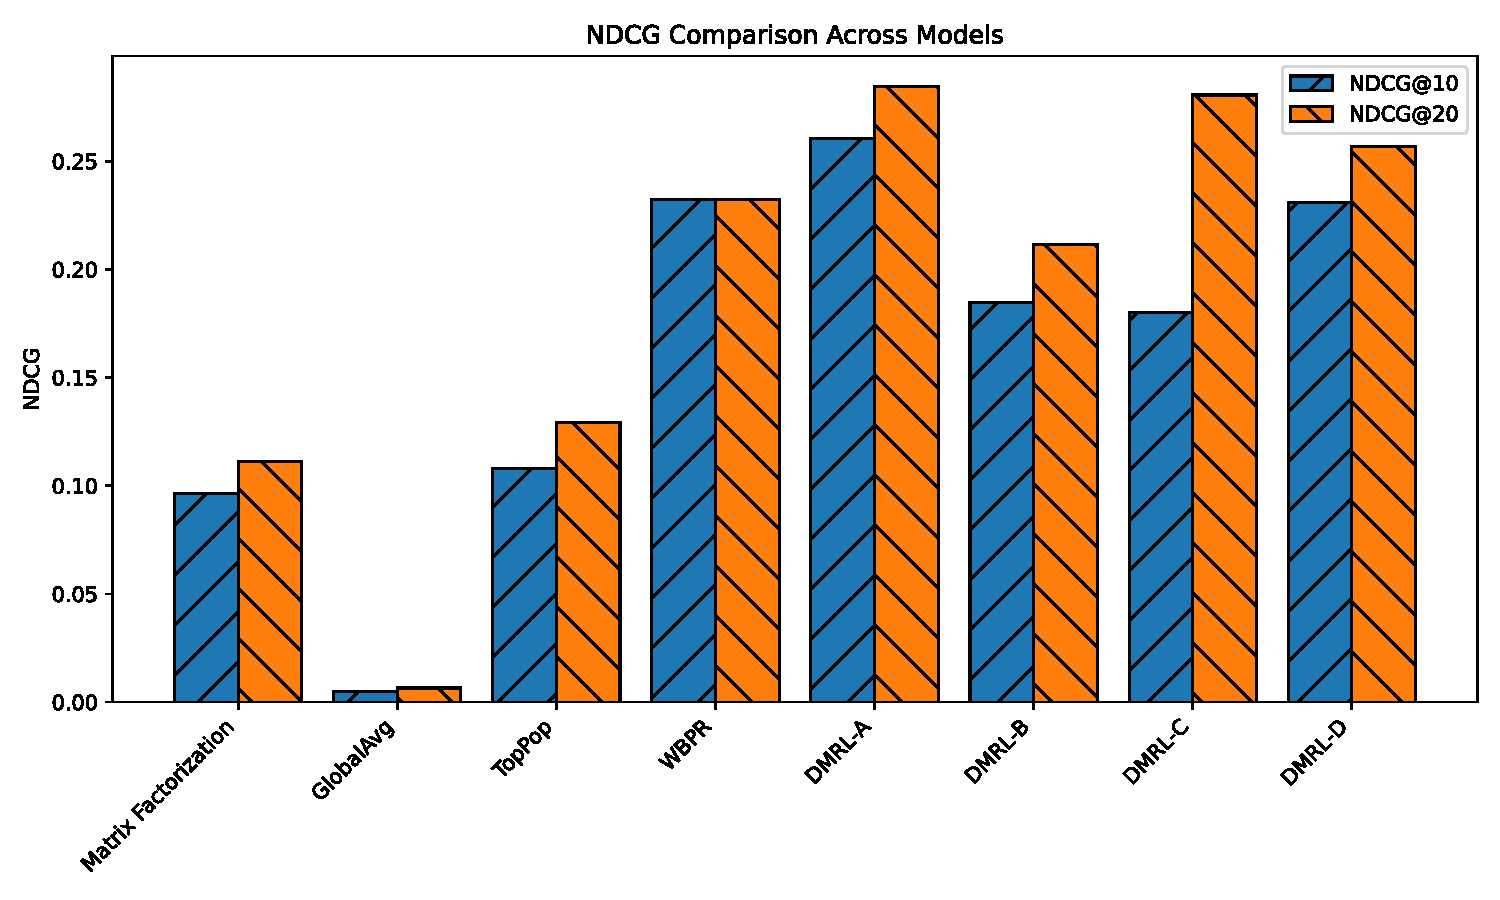
\includegraphics[width=\textwidth]{images/ndcg_comparison.pdf}
        \end{minipage}
        \hfill
        \begin{minipage}{0.48\textwidth}
            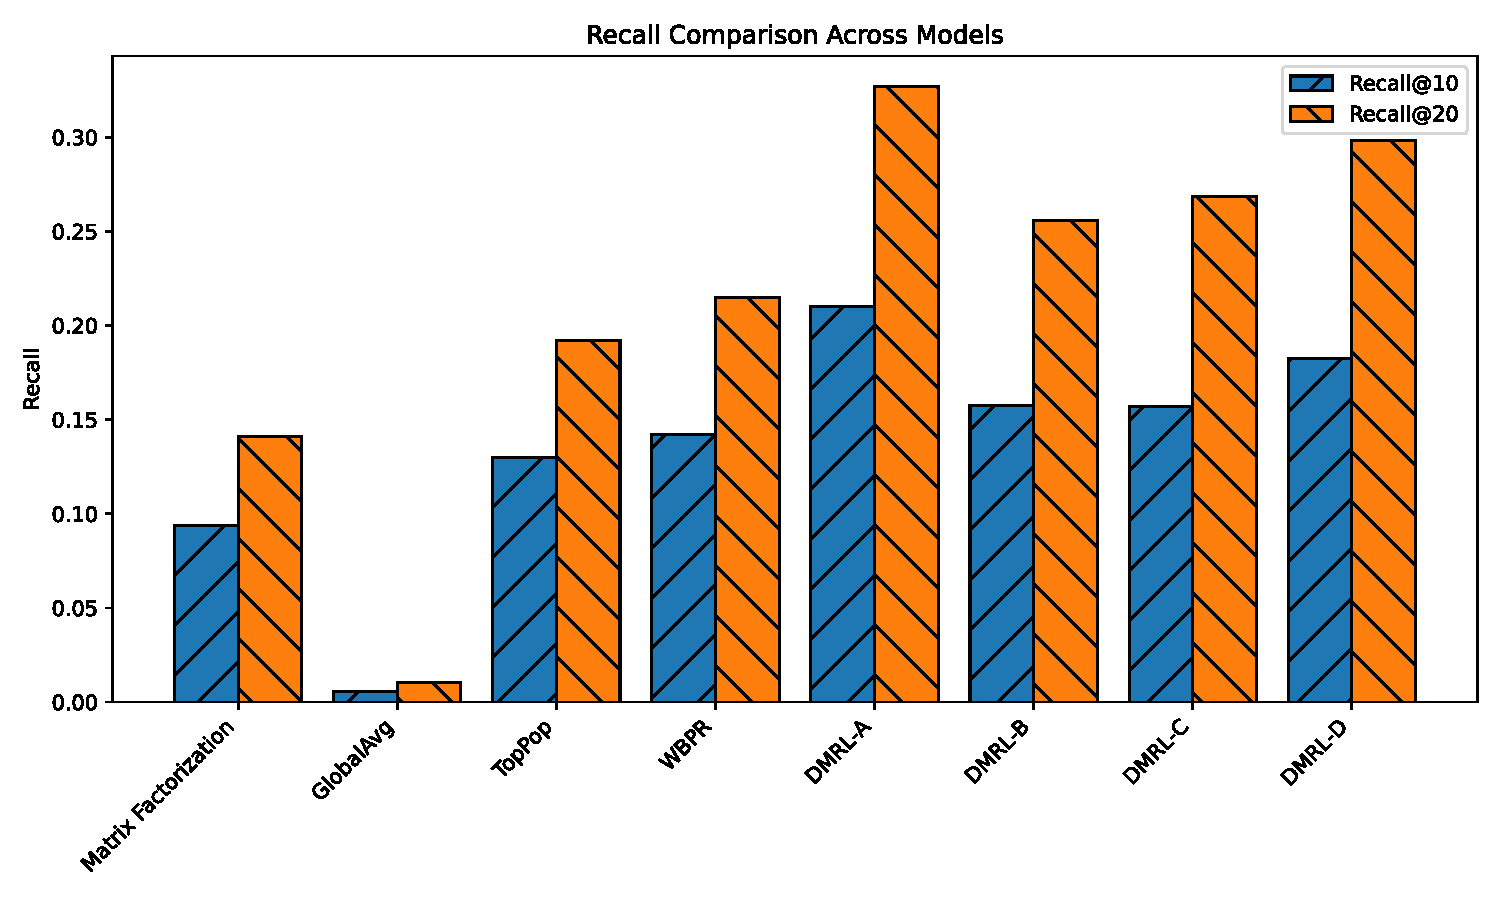
\includegraphics[width=\textwidth]{images/recall_comparison.pdf}
        \end{minipage}
    \end{figure}
\end{frame}

\begin{frame}{Similitud coseno para Toy Story}
    \begin{figure}
        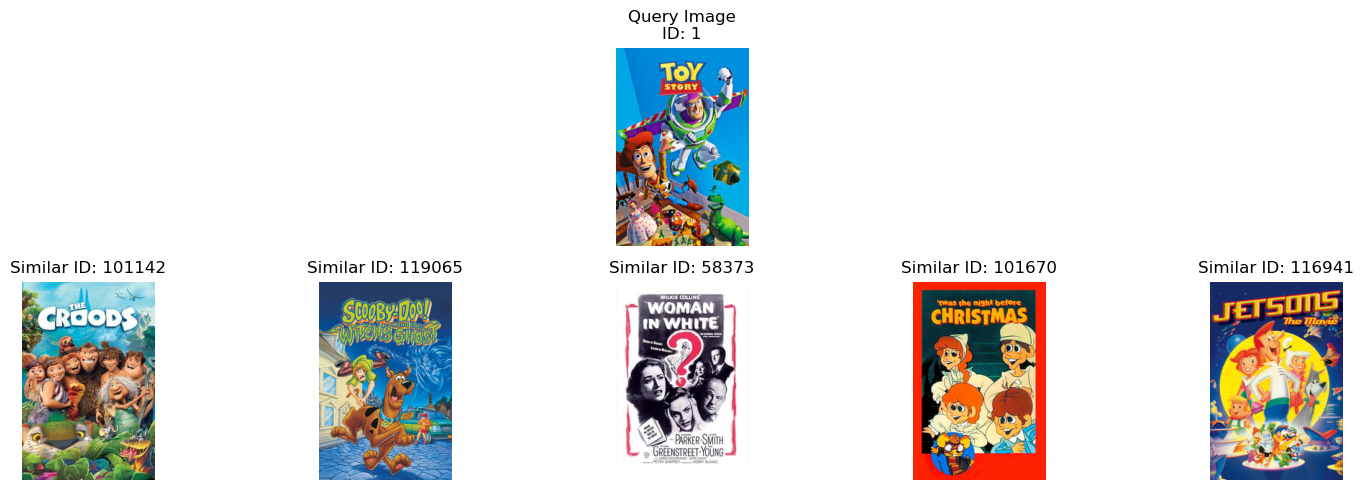
\includegraphics[width=\textwidth]{images/vgg16_cnn_nopca.png}
    \end{figure}
\end{frame}

\begin{frame}{Similitud coseno con PCA}
    \begin{minipage}{0.48\textwidth}
        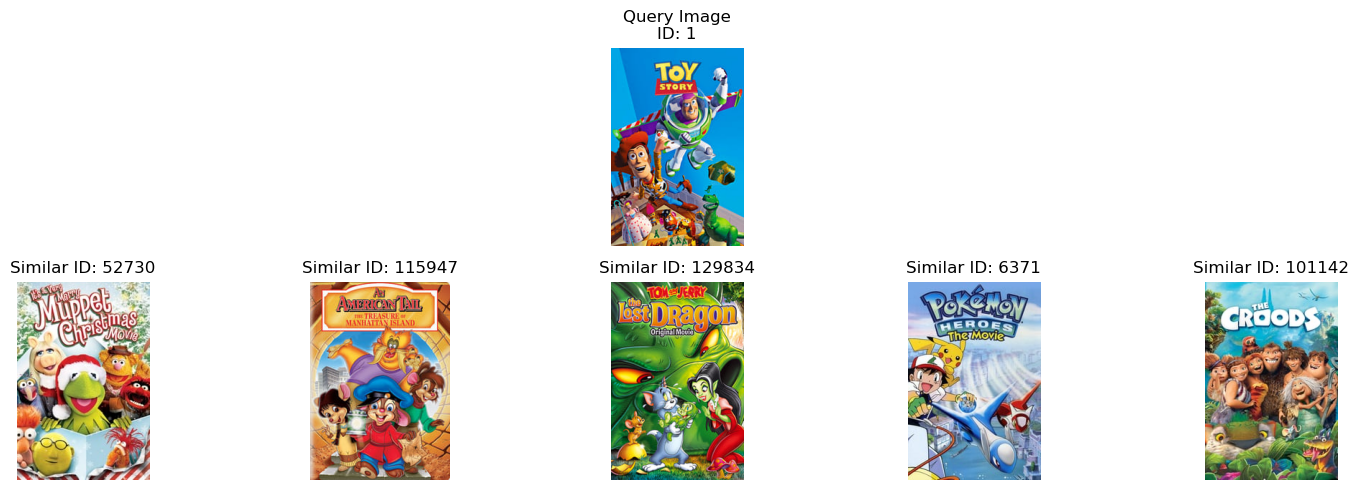
\includegraphics[width=\textwidth]{images/vgg16_cnn.png}
    \end{minipage}
    \hfill
    \begin{minipage}{0.48\textwidth}
        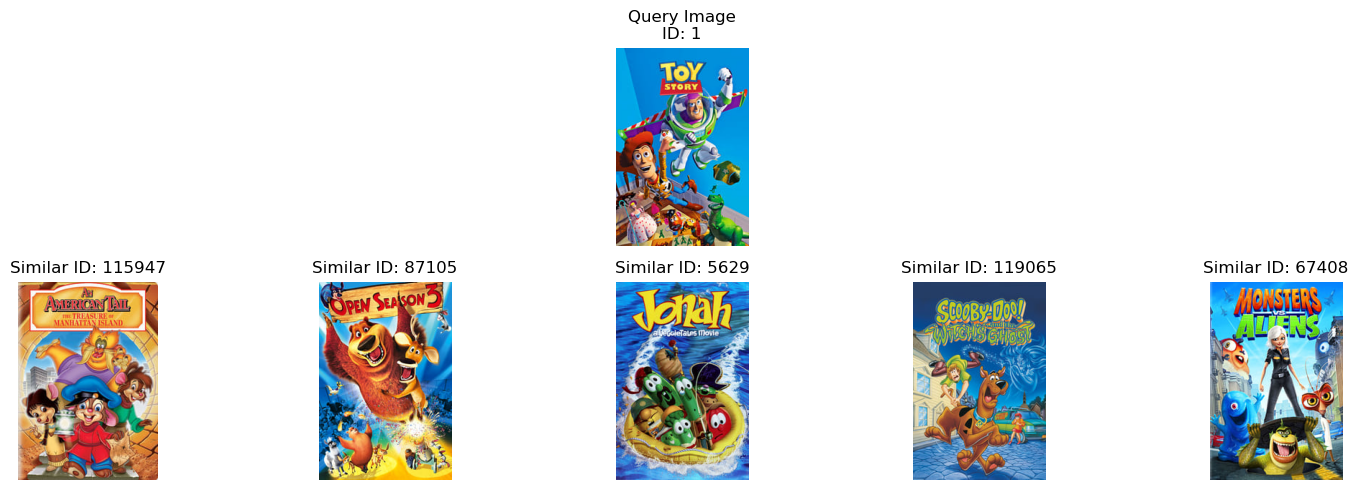
\includegraphics[width=\textwidth]{images/vgg16_fc2.png}
    \end{minipage}
\end{frame}

% Architectural Considerations
\section{Consideraciones arquitectónicas}
\begin{frame}{Propuesta arquitectónica}
    \begin{center}
        \includegraphics[width=0.9\textwidth]{images/tfm-arch.drawio.pdf}
    \end{center}
    \caption{Arquitectura propuesta para despliegue en producción.}
\end{frame}

% Future Work
\section{Trabajo futuro}
\begin{frame}{Trabajo futuro}
    \textbf{Posibles direcciones:}
    \begin{itemize}
        \item Extender el sistema a datasets más grandes como MovieLens-20M.
        \item Integrar modalidades adicionales como audio o reseñas.
        \item Validar en entornos reales mediante pruebas A/B.
    \end{itemize}
\end{frame}

% Conclusions
\section{Conclusiones}
\begin{frame}{Conclusiones}
    \begin{itemize}
        \item Los datos multimodales mejoran significativamente la personalización.
        \item DMRL aborda problemas clave como cold start y long tail.
        \item Consideraciones para su despliegue en sistemas de producción.
    \end{itemize}
\end{frame}

% Closing Slide
\begin{frame}{¡Gracias!}
    \begin{center}
        ¿Preguntas?
    \end{center}
\end{frame}


\end{document}